\documentclass[a4paper]{article}
\usepackage{tikz}
\usepackage{siunitx}
\usepackage{xcolor}
\usepackage{pgfplots}
\usepackage{amsmath}
\usepackage{cleveref}

\usetikzlibrary{calc}

\tikzset{
	polaraxis/.style={dashed,thick},%
	nauvis/.style={very thick},%
	equator/.style={dotted,very thick},%
	latitude/.style={green,thick},%
	daynightline/.style={dash dot},%
	day/.style={yellow,fill opacity=0.2},%
	night/.style={blue!50!red,fill opacity=0.2},%
	angle/.style={thin},%
	dimension/.style={|-|,shorten <=0.05cm,shorten >=0.05cm},%
}
%\def\thetaangle{20}
%\def\phiangle{63.55}
\def\thetaangle{17}
\def\phiangle{62}


\title{A geometrical and astronomical exploration of Nauvis}
\author{gustaphe}

\begin{document}
\maketitle

What can we know about Nauvis? Quite a lot. First off: There appears to be no seasons, or at least no noticeable changes in day length have happened during the five Earth-years that I've played this game, so if there is seasonal variation it's small, slow or both. Either the player is on the equator of Nauvis, or Nauvis' axis of rotation stays at a constant angle \(\theta\) from its axis of revolution around its sun (see \cref{fig:seasons}).


\begin{figure}
	\centering
	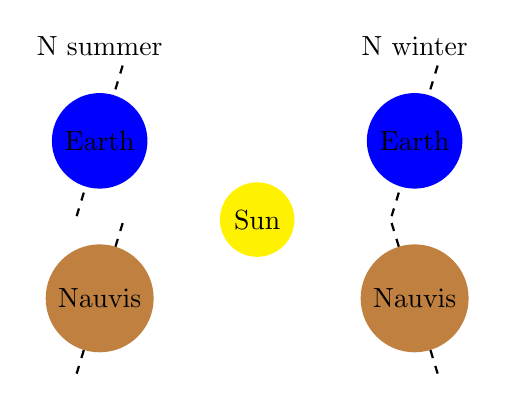
\begin{tikzpicture}
		\node[fill=yellow,circle] at (0,0) {Sun};
		\draw[polaraxis] %
		(-2,1) node[fill=blue,circle] {Earth} +(90-\thetaangle:1) -- +(270-\thetaangle:1) +(0,1.2) node {N summer}%
		(2,1) node[fill=blue,circle] {Earth} +(90-\thetaangle:1) -- +(270-\thetaangle:1) +(0,1.2) node {N winter}%
		(-2,-1) node[fill=brown,circle] {Nauvis} + (90-\thetaangle:1) -- +(270-\thetaangle:1)%
		(2,-1) node[fill=brown,circle] {Nauvis} + (90+\thetaangle:1) -- +(270+\thetaangle:1)%
		;
	\end{tikzpicture}
	\caption{Earth's seasons, vs Nauvis' constant summer. Dashed line is the polar axis, around which the planet spins diurnally}\label{fig:seasons}
\end{figure}


\begin{figure}
	\centering
	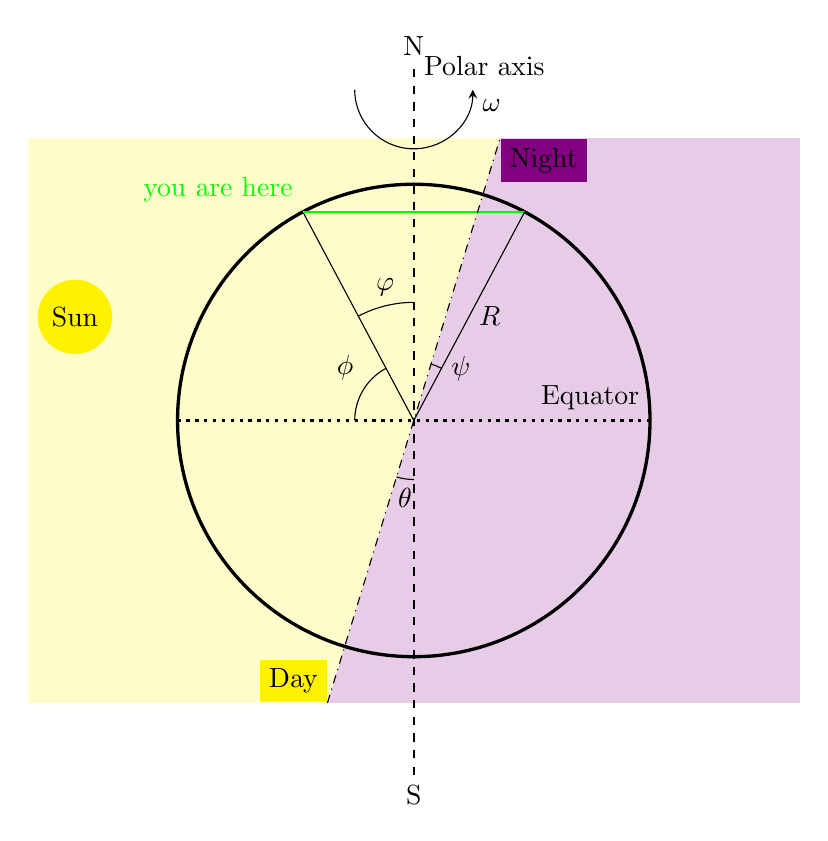
\begin{tikzpicture}[%
		x=3cm,y=3cm,%
		];
		\fill[day] (270-\thetaangle:1.25) -- (90-\thetaangle:1.25) -- +(-2,0) |- cycle;
		\fill[night] (270-\thetaangle:1.25) -- +(2,0) |- (90-\thetaangle:1.25) -- cycle;
		\path (270-\thetaangle:1.25) node[fill=yellow,above left] {Day} (90-\thetaangle:1.25) node[fill=blue!50!red,below right] {Night} (180-\thetaangle:1.5) node[circle,fill=yellow]{Sun};
		\draw[nauvis] (0,0) circle (1);
		\draw[polaraxis] (0,-1.5) node[below] {S} -- (0,1.5) node[right]{Polar axis} node[above]{N};
		\draw[equator] (-1,0) -- (1,0) node[above left]{Equator};
		\draw[-stealth] (0,1.4) +(180:0.25) arc (180:360:.25) node[below right] {\(\omega\)};
		\draw (0,0) -- (180-\phiangle:1);
		\draw[angle] (180-\phiangle:0.25) arc (180-\phiangle:180:0.25) node[midway,above left] {\(\phi\)};
		\draw[latitude] (\phiangle:1) -- (180-\phiangle:1) node[above left]{you are here};
		\draw[daynightline] (270-\thetaangle:1.25) -- (90-\thetaangle:1.25);
		\draw[angle] (270-\thetaangle:0.25) arc (270-\thetaangle:270:0.25) node[midway,below]{\(\theta\)};
		\draw (0,0) -- (\phiangle:1) node[midway,right]{\(R\)};
		\draw[angle] (90-\thetaangle:0.25) arc (90-\thetaangle:\phiangle:0.25) node[right] {\(\psi\)};
		\draw[angle] (180-\phiangle:0.5) arc (180-\phiangle:90:0.5) node[midway,above] {\(\varphi\)};
	\end{tikzpicture}
	\caption{Definitions of some useful angles on Nauvis -- \(\phi\) is the traditional definition of latitude, with \(\varphi\) being the same angle but defined from the pole instead of the equator. \(\theta\) is the tilt angle between the polar axis and the plane orthogonal to the Sun -- Nauvis vector (the ``day -- night plane''). Marked in green is the latitude circle around which the player character moves}\label{fig:definitions}
\end{figure}

\begin{figure}
	\centering
	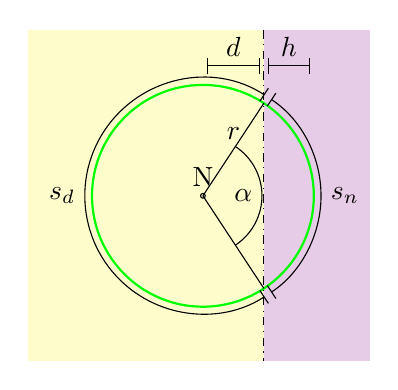
\begin{tikzpicture}[%
		x=3cm,y=3cm,%
		]
		\fill[day] ({sin(\phiangle)*sin(\thetaangle)},0) +(0,0.7) rectangle +(-1,-0.7);
		\fill[night] ({sin(\phiangle)*sin(\thetaangle)},0) +(0,0.7) rectangle +(0.45,-0.7);
		\draw (0,0) circle(0.01) node[above]{N};
		\draw[latitude] (0,0) circle ({cos(\phiangle)});
		\draw[daynightline] ({sin(\phiangle)*sin(\thetaangle)},0) +(0,0.7) -- +(0,-0.7);
		\draw (0,0) -- ({acos(tan(\phiangle)*sin(\thetaangle))}:{cos(\phiangle)}) node[midway,above] {\(r\)} (0,0) -- ({-acos(tan(\phiangle)*sin(\thetaangle))}:{cos(\phiangle)});
		\draw[angle] ({acos(tan(\phiangle)*sin(\thetaangle))}:0.25) arc ({acos(tan(\phiangle)*sin(\thetaangle))}:{-acos(tan(\phiangle)*sin(\thetaangle))}:0.25) node[midway,left]{\(\alpha\)};
		\draw[dimension] ({acos(tan(\phiangle)*sin(\thetaangle))}:0.5) arc ({acos(tan(\phiangle)*sin(\thetaangle))}:{-acos(tan(\phiangle)*sin(\thetaangle))}:0.5) node[midway,right]{\(s_n\)};
		\draw[dimension] ({acos(tan(\phiangle)*sin(\thetaangle))}:0.5) arc ({acos(tan(\phiangle)*sin(\thetaangle))}:{-acos(tan(\phiangle)*sin(\thetaangle))+360}:0.5) node[midway,left]{\(s_d\)};
		\draw[dimension] (0,0.55) -- ({sin(\phiangle)*sin(\thetaangle)},0.55) node[midway,above]{\(d\)};
		\draw[dimension] ({sin(\phiangle)*sin(\thetaangle)},0.55) -- ({cos(\phiangle)},0.55) node[midway,above]{\(h\)};
	\end{tikzpicture}
	\hspace{1cm}
	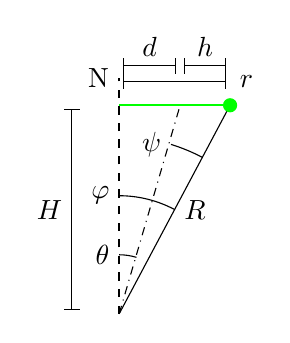
\begin{tikzpicture}[x=3cm,y=3cm]
		\draw (0,0) -- (\phiangle:1) node[midway,right]{\(R\)};
		\draw[daynightline] (0,0) -- ({sin(\phiangle)*sin(\thetaangle)},{sin(\phiangle)});
		\draw[polaraxis] (0,0) -- (0,1) node[above,left]{N};
		\fill[latitude] (\phiangle:1) circle (0.03);
		\draw[latitude] (\phiangle:1) -- (0,{sin(\phiangle)});
		\draw[dimension,yshift={0.3cm}] (0,{sin(\phiangle)}) -- (\phiangle:1) node[right]{\(r\)};
		\draw[dimension,yshift={0.5cm}] (0,{sin(\phiangle)}) -- ({sin(\phiangle)*sin(\thetaangle)},{sin(\phiangle)}) node[midway,above]{\(d\)};
		\draw[dimension,yshift={0.5cm}] ({sin(\phiangle)*sin(\thetaangle)},{sin(\phiangle)}) -- (\phiangle:1) node[midway,above]{\(h\)};
		\draw[angle] (0,0.25) node[left]{\(\theta\)} arc (90:{90-\thetaangle}:0.25);
		\draw[angle] (0,0.5) node[left]{\(\varphi\)} arc (90:{\phiangle}:0.5);
		\draw[angle] ({90-\thetaangle}:0.75) node[left]{\(\psi\)} arc ({90-\thetaangle}:\phiangle:0.75);
		\draw[dimension,xshift={-0.6cm}] (0,0) -- (0,{sin(\phiangle)}) node[midway,left]{\(H\)};
	\end{tikzpicture}

	\caption{(left) Intersection of \cref{fig:definitions} along the plane spanned by the player's latitude circle. (right) More detailed version of \cref{fig:definitions} for trigonometrical reasoning}\label{fig:intersection}
\end{figure}


The diurni (day+night) on Nauvis last an amount of time \(T=\SI{25000}{ticks}\), during which the days (mid-sunrise -- mid-sunset) last \(T_d=\SI{17500}{ticks}\). If we were on the equator, days and nights would be equal in length, so we're not. That leaves a constant \(\theta\). \Cref{fig:definitions} illustrates the involved angles.

The unequal day and night lengths are explained by a latitude (angle from the equator) \(\phi\). As Nauvis rotates around its axis, the player moves around a latitude circle, dipping in and out of the night time zone, but due to \(\theta\), the day-night plane doesn't cut this latitude circle by its diameter, rather cutting a cord (see \cref{fig:intersection}).

Assuming a constant spinning rate \(\omega\), the day fraction of the diurnus should equal the fraction of the latitude circle in the day zone,
\[
	\frac{T_d}{T}=\frac{s_d}{s_d+s_n}=1-\frac{\alpha}{\tau}
\]

By some basic trigonometry on \cref{fig:intersection}, we get \(d=H\tan\theta\), \(r=H\tan\varphi\), 
\[
	\begin{gathered}
		\alpha=2\arccos\left(\frac{d}{r}\right)=2\arccos\left(\frac{\tan\theta}{\tan\varphi}\right) \\
		\Longrightarrow \frac{\tan\theta}{\tan\varphi}=\cos\left(\frac{\tau}{2}-\frac{T_d}{2T}\tau\right)=-\cos\left(\frac{T_d}{2T}\tau\right)\approx0.59
	\end{gathered}
\]

Now there's a degree of freedom in our choice of \(\theta\) and \(\varphi\), which we cannot resolve based on the well defined numbers in game. Instead we have to turn to some more subjective measurement. We can use the length of the engineer's shadow for this. The trigonometry is displayed in \cref{fig:shadow}. If we assume that this is supposed to represent the shadow at mid-day (it doesn't change over time in game, \emph{literally unplayable}). The perspective is difficult, but as a rough guesstimate, we can say that the shadow is as long as the engineer is tall, \(L_s=L\). Now \(\frac{\tau}{4}-\theta-\varphi=\arctan(1)=\frac{\tau}{8}\), which resolves our degree of freedom.
\[
	\tan\theta=0.59\tan\varphi=0.59\tan\left(\frac{\tau}{8}-\theta\right)
\]

We can solve this numerically, as in \cref{fig:numerics}, which gives \(\theta=0.301\) and \(\varphi=0.484\). In conclusion: If the engineer's shadow is as long as he is tall, the game is set at latitude \(\phi=\frac{\tau}{4}-\varphi=\SI{62}{\degree}\), about the same latitude as the Faroe Islands on Earth, and Nauvis has a constant tilt of \(\theta=\SI{17}{\degree}\).

\begin{figure}
	\centering
	\begin{tikzpicture}[x=2cm,y=2cm]
		% Planet {{{
		\draw (0,0) circle(1);
		\draw[green,very thick] (180-\phiangle:1) -- (180-\phiangle:1.075);
		\draw[very thick,night] (180-\phiangle:1) -- +(90-\phiangle:0.075);
		\draw (0,0) -- (180-\phiangle:1);
		\draw[polaraxis] (0,-1.5) node[below] {S} -- (0,1.5) node[above]{N};
		\draw[daynightline] (-\thetaangle:1.5) -- (180-\thetaangle:1.5) (0,0.8) -- ($(180-\thetaangle:1.5)+(0,0.8)$);
		\draw[angle] (-90:0.5) arc (-90:-\thetaangle:0.5) node[above]{\(\frac{\tau}{4}-\theta\)} %
		(180-\phiangle:0.5) arc (180-\phiangle:90:0.5) node[right]{\(\varphi\)}%
		(180-\phiangle:1.075) + (-\phiangle:0.45) node[left] {\(\frac{\tau}{4}-\theta-\varphi\)} arc (-\phiangle:-\thetaangle:0.45);
		;
		\draw[very thin,blue] (180-\phiangle:0.95) -- ++(90-\phiangle:0.1) -- ++(180-\phiangle:0.2) -- ++(270-\phiangle:0.2) -- ++(-\phiangle:0.2) -- cycle;
		% }}}
	\end{tikzpicture}
	\hspace{1cm}
	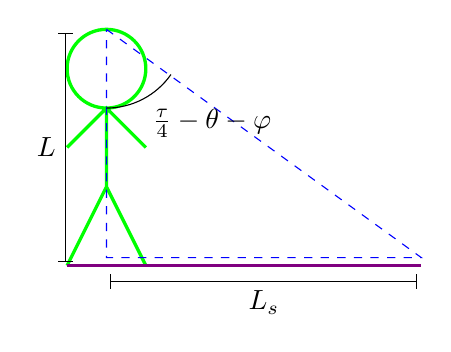
\begin{tikzpicture}
		% Stick figure {{{
		\draw[green,very thick] (0,0) +(0.5,0) -- +(0,1) -- +(-0.5,0) ++(0,1) -- ++(0,1) +(0.5,-0.5) -- +(0,0) -- +(-0.5,-0.5) ++(0,0.5) circle(0.5);
		% }}}
		% Shadow {{{
		\draw[very thick,night] (-0.5,0) -- (4,0);
		% }}}
		\draw[dashed,blue] (0,3) -- (4,0.1) -- (0,0.1) -- cycle;
		\draw[angle] (0,3) +(-90:1) arc (-90:-35:1) node[midway,below right] {\(\frac{\tau}{4}-\theta-\varphi\)};
		\draw[dimension,yshift={-0.2cm}] (0,0) -- (4,0) node[midway,below] {\(L_s\)};
		\draw[dimension,xshift={-0.52cm}] (0,0) -- (0,3) node[midway,left] {\(L\)};
	\end{tikzpicture}
	\caption{(left) Relevant geometry for calculating \(\theta\) and \(\phi\) from the shadow length of a person. (right) detail from the picture on the left}\label{fig:shadow}
\end{figure}

\begin{figure}
	\centering
	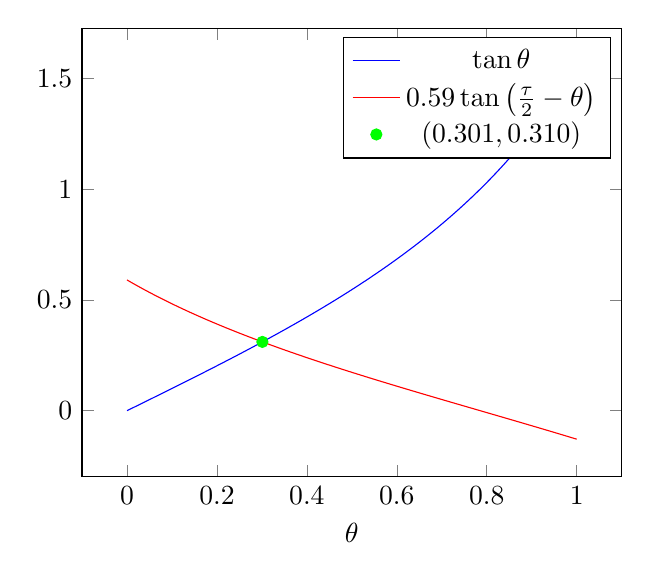
\begin{tikzpicture}
		\begin{axis}[%
			xlabel=\(\theta\),%
			]
			\addplot[blue,domain=0:1,samples=101] {tan(deg(x))};
			\addlegendentry{\(\tan\theta\)}
			\addplot[red,domain=0:1,samples=101] {0.59*tan(deg(pi/4-x))};
			\addlegendentry{\(0.59\tan\left(\frac{\tau}{2}-\theta\right)\)}
			\addplot[green,only marks] coordinates {(0.301018,0.31045239)};
			\addlegendentry{\((0.301,0.310)\)}
		\end{axis}
	\end{tikzpicture}
	\caption{Numerical solution to the trigonometric expression}\label{fig:numerics}
\end{figure}


\end{document}

